\section {Sulfur Dioxide Bonding Coordinations}

The bonding coordination of the surface \suldiox~was determined at each timestep of the simulations. Figure \ref{fig:bonding-coordinations} shows the distribution of coordinations of the surface \suldiox, by percent of simulation time, across all the simulations for both the cold (blue) and hot (red) trajectories. A first visual inspection clearly indicates the two most common coordinations: ``S'' and ``SO'', followed by the unbound coordination, and ``SOO''. This trend holds at both temperatures. Also, a \suldiox~configuration with bonds forming solely through the oxygens without any sulfur interactions, or any configuration with more than a single interaction the the sulfur atom are rare in comparison to the single sulfur coordinations. These less common coordinations likely form as transitory configurations when the waters briefly move closer or further away from the surface \suldiox.

The distribution paints a likely picture of the surface adsorption process of a \suldiox~first coming in contact with surface waters. Starting in an unbound state, two methods of initial contact are possible: through the \suldiox-sulfur of through one of the oxygens. Because the population of non-sulfur interactions (i.e. ``O'', ``OO'', ``OOO'', etc.) only account for 3\% of all the configurations sampled, either there is a very brief transition state where the \suldiox~first binds through an oxygen and then quickly adds, or switches to a sulfur interaction with the surface waters, or the first contact is made through the sulfur atom. Because the ``S'' coordination has such a large population, accounting for 35\% of the trajectories in the cold systems, and 32\% in the hot systems, it is most likely that the first binding contact to the waters is through the \suldiox~sulfur to a water oxygen. Furthermore, once in the ``S'' coordination, the \suldiox~can either unbind, add a second sulfur interaction, or bind through an oxygen. The histogram of Figure \ref{fig:bonding-coordinations} suggests that the preferred route is to further coordinate through an oxygen to achieve the ``SO'' coordination. ``SO'' accounts for 35\% of the cold coordinations, and 36\% of the hot trajectories. Binding to a second oxygen to the ``SOO'' coordination (7\% of the cold, 12\% of the hot systems) is less likely than losing an interaction through an oxygen back to the ``S'' coordination.

We thus have a likely route for adsorption and binding of an unbound \suldiox~to a water surface. The unbound \suldiox~initially binds mostly to a water through the sulfur atom, and then will either unbind, or add an oxygen interaction to oscillate between unbound, ``S'', and ``SO'' coordinations. It may then undergo brief sojourns to other coordinations because of the motions and rearrangements of the surface water molecules. These brief transitory coordinations are overwhelmed by the dominant ``S'' and ``SO'' states. The most probable deviation from those two coordinations is to the ``SOO'', where a second oxygen interaction is formed. Otherwise the \suldiox~unbinds from the surface to repeat the adsorption process.

Baer et al performed this coordination analysis for their single-temperature study, but discriminating between \suldiox~binding through the two different oxygens. They concluded that there is asymmetric hydrogen bonding through the \suldiox~oxygens, with one binding more often than the other. This is supported by the findings here where all the double oxygen coordinations (i.e. ``OO'', ``SOO'', etc.) represent a much lower percentage of the coordinations than the single oxygen counterparts (i.e. ``O'', ``SO'', etc.). 

%To further assess the effect of temperature on \suldiox~behavior we turn to analysis of the bonds formed between \suldiox~and the water surface. The bonding coordinations were determined for the \suldiox~based on the bondlength criteria noted in the introduction. Bonds formed between \suldiox-sulfur and \wat-oxygen are labeled 'S' coordinated, and bonds formed between \suldiox-oxygen and \wat-hydrogen are labeled 'O' coordinated. For each bond an additional letter label is appended to the coordination. For example, an 'SOO' coordinated \suldiox~forms three bonds to waters: two bonds are formed through the \suldiox-oxygens, and one through the \suldiox~sulfur. This naming scheme is taken from a similar convention used for describing water bonding interactions, but applied now to the \suldiox~molecule.\cite{Buch2005} 

%Figure \ref{fig:so2-bonding-coordinations} shows the distribution of bonding coordinations throughout the set of simulated trajectories for both the cold and hot temperatures. The two most common coordination types are the S and SO, followed by a completely unbound \suldiox~molecule. Bonding is primarily found through the \suldiox-sulfur atom, with higher coordinationsThe distribution shows that the \suldiox~mostly forms one or two bonding interactions with the waters. The bonding of the \suldiox~at both low and high temperatures follows similar trends, however the higher temperature shifts the distribution of coordinations slightly to forming more bonds than the cold temperature \suldiox. Figure \ref{fig:coordination-breakdown} breaks down the coordination distribution to show more details of the \suldiox~interactions.

%The total number of bonds formed to the \suldiox~are shown in the top plot of figure \ref{fig:coordination-breakdown}. The \suldiox~spends more than 70\% of the trajectories forming single or double interactions with surface waters. The center and bottom plots of figure \ref{fig:coordination-breakdown} show the distribution of bonds formed through the \suldiox~sulfur and oxygen atoms, respectively. The sulfur interaction distribution (center) shows the \suldiox~clearly spending most of the simulations forming a single bond through the sulfur atom. This supports the overall distributions heavily weighted by the S and SO coordination types. Looking at the oxygen interaction distribution plot (bottom) of figure \ref{fig:coordination-breakdown}, the oxygen remains mostly unbound or singly bound. By increasing the temperature the amount of unbound oxygen coordinations decreases 10\%, but the increase in the singly bound state is only by 4\%, while the double oxygen interactions increase by 6\% over the colder temperature distribution. Higher temperatures shift the distribution of interactions with \suldiox~to higher coordination types.

%The sfg experiment performed by our group on \suldiox~surface adsorption suggested an SO coordination type based on...\cite{Tarbuck2005,Tarkbuch2006} This was further supported by DFT simulations of single surface \suldiox~molecules bound to water at room temperature.\cite{Baer2010} Our simulations show that the SO interaction type is nearly as prevalent as the single S-type coordination at both temperatures. The colder temperature favors the single bond to the \suldiox~through the sulfur atom more than the high temperature, but the increase in coordination number of the \suldiox~is subtle and does not drastically change with temperature.

% Figure showing all the different types of so2 coordinations
%\begin{figure}[h!]
	%\begin{center}
		%\includegraphics[scale=1.0]{images/coordination/so2-bonding-coordinations.png}
		%\caption{Distribution of bonding coordinations of the surface \suldiox~molecule. Each set of bars represents the amount of time spent in the particular coordination type, including the unbound coordination. The results for the cold (blue) and hot (red) temperatures are shown together. At the high temperature the \suldiox~bonding becomes more complex with more bonds to the sulfur and oxygen atoms. The lower coordination states are more dominated in the cold temperature. The naming scheme is similar to that of a previous scheme for water coordinations,\cite{Buch2005} applied to the \suldiox~molecule.}
		%\label{fig:so2-bonding-coordinations}
	%\end{center}
%\end{figure}


%\begin{figure}[h!]
	%\begin{center}
		%\includegraphics[scale=1.0]{images/coordination/coordination-breakdown.png}
		%\caption{Bonding coordinations of the \suldiox~broken down into specific interactions. The total number of bonds to the molecule (top) are shown regardless of coordination type. The total number of bonds through either the sulfur atom (center) or through both of the oxygens (bottom). The \suldiox~primarily forms one or two bonds to the surface waters. The sulfur atom mostly bonds to a single water oxygen. Between the two \suldiox~oxygen atoms, the molecule mostly does not bond to the water hydrogens, or forms a single hydrogen-bond.}
		%\label{fig:coordination-breakdown}
	%\end{center}
%\end{figure}


\subsection {Temperature Effects on Bonding Coordinations}

The binding behavior of the \suldiox~is altered by changing the temperature of the system, as evidenced in the shift in coordination populations of Figure \ref{fig:bonding-coordinations} from cold to hot. In the cold temperature, the unbound, single oxygen, and ``S'' coordinations are more populated than in the hot systems. The increased temperature causes all the coordinations with a single sulfur interaction or more (with the exception of ``S'') to increase over the equivalent cold temperature coordination populations. We see that the cold \suldiox~spends nearly twice as much time unbound, and only slightly more time in the ``S'' coordination. Most of the unbound population in the hot simulations appears to have shifted to the states with double-oxygen and double-sulfur coordinations. Figure \ref{fig:coordination-breakdown} shows the distribution of the number of bonds through the \suldiox~oxygens (left) and through the \suldiox~sulfur (right). When comparing from cold to hot distributions, the greatest shift occurs in the number of \suldiox~oxygen bonds as the hot \suldiox~has more multiply-bound oxygens (double and triple interactions). The increased temperature allows the \suldiox~oxygens to bind to more water hydrogens than in the cold systems.

These increased binding through the \suldiox~oxygens at the hot temperatures should have a visible effect on the radial distribution function (RDF) between \suldiox-oxygen and water-hydrogen. Figure \ref{fig:rdf} shows the RDF of the \suldiox~sulfur and oxygen atoms with their water bonding partners, water oxygen and hydrogen, respectively, at both cold and hot temperatures. Both the first and second peaks of the O$_{SO_2}$-H$_{H_2O}$ RDF increase at the higher temperature, indicating a large number of water hydrogens near the \suldiox~oxygens in both hydration shells. This corroborates the increased coordination through the \suldiox~oxygens to the surface waters at the higher temperature.

The populations of the single-oxygen coordinations are similar at both temperatures, somewhat contradicting the results of the RDF. We expect an increase of all \suldiox-oxygen interactions with surface water hydrogens, but the non-sulfur coordinations do not obey this trend. This indicates that the non-sulfur coordinations do not behave as most of the other coordinations, and their small contribution to the overall population in the distribution of Figure \ref{fig:bonding-coordinations} indicates that they are anomalous, or only briefly encountered during the simulations.

The same temperature effect of shifting population to higher coordinations also manifests in the \suldiox~sulfur. The single-``S'' coordinations have similar populations at both temperatures, but the change from cold to hot temperature shifts the unbound \suldiox~coordinations up towards to the doubly-bound sulfur coordinations (i.e. ``SS'', ``SSO'', etc.). The increased temperature causes more binding to the \suldiox~by allowing for multiple bonds through both the \suldiox~sulfur, and through the oxygens. Thus, the hotter temperature allows for increased coordination of the \suldiox~to the water surface.

When the \suldiox~is on the cold water surface, the ``S'' and ``SO'' coordination populations are nearly equally represented. As the temperature increases to the hot system, the ``S'' coordination decreases, while the ``SO'' increases. We see from the RDFs that colder temperatures favor binding through the \suldiox~sulfur because of the larger first peak in the S$_{SO_2}$-O$_{H_2O}$ RDF. From this increase we expect the ``S''-coordinated \suldiox~to be more prevalent at cold temperatures, as is the case for the coordination distribution. However, the O$_{SO_2}$-H$_{H_2O}$ RDF indicates increased hydrogen bonding through the \suldiox~oxygens at higher temperatures manifested by a larger first peak in Figure \ref{fig:rdf} for the hot temperature. Thus the minimally ``SO''-coordinated distributions (those with at least a single bond to an oxygen and the sulfur, i.e. ``SO'', ``SSO'', ``SSOO'', etc.) are more prevalent at the high temperature. Overall, we find evidence from both the bonding coordination distribution, and from the RDFs to suggest a modified bonding behavior at different temperatures. At an increased temperature the surface \suldiox~binds more through its oxygens than the cold counterpart. However, like the \suldiox~in the cold temperature, it likely has a persistent interaction through the sulfur atom to a neighboring water oxygen throughout most of the simulated trajectories.
